\documentclass[12pt, titlepage]{article}

\usepackage{booktabs}
\usepackage{tabularx}
\usepackage{hyperref}
\usepackage{float}
\usepackage{graphicx}
\hypersetup{
    colorlinks,
    citecolor=black,
    filecolor=black,
    linkcolor=red,
    urlcolor=blue
}
\usepackage[round]{natbib}

\input{../Comments}
%% Common Parts

\newcommand{\progname}{Baja Dynamics} % PUT YOUR PROGRAM NAME HERE
\newcommand{\authname}{Team \#17, Team Name
\\ Grace McKenna
\\ Travis Wing
\\ Cameron Dunn
\\ Kai Arseneau} % AUTHOR NAMES                  

\usepackage{hyperref}
    \hypersetup{colorlinks=true, linkcolor=blue, citecolor=blue, filecolor=blue,
                urlcolor=blue, unicode=false}
    \urlstyle{same}
                                


\begin{document}

\title{Verification and Validation Report: \progname} 
\author{\authname}
\date{\today}
	
\maketitle

\pagenumbering{roman}

\section{Revision History}

\begin{tabularx}{\textwidth}{p{3cm}p{2cm}X}
\toprule {\bf Date} & {\bf Version} & {\bf Notes}\\
\midrule
Date 1 & 1.0 & Notes\\
Date 2 & 1.1 & Notes\\
\bottomrule
\end{tabularx}

~\newpage

\section{Symbols, Abbreviations and Acronyms}

\renewcommand{\arraystretch}{1.2}
\begin{tabular}{l l} 
  \toprule		
  \textbf{symbol} & \textbf{description}\\
  \midrule 
  T & Test\\
  \bottomrule
\end{tabular}\\

\wss{symbols, abbreviations or acronyms -- you can reference the SRS tables if needed}

\newpage

\tableofcontents

\listoftables %if appropriate

\listoffigures %if appropriate

\newpage

\pagenumbering{arabic}

This document ...

\section{Functional Requirements Evaluation}

\section{Nonfunctional Requirements Evaluation}

\subsection{Usability}
		
\subsection{Performance}

\subsection{etc.}
	
\section{Comparison to Existing Implementation}	

Not applicable for this project.
\section{Unit Testing}

\subsection{Back End Unit Testing}
The back end was fully covered by unit tests except for a several files which were not suited for unit testing as they were mainly constants or did not provide functionality that could be tested. \\
\\
The test structure that was created was to essentially mirror how the codebase is organized. There is a test folder which houses all the tests, then inside that there is a simulations and utils folder which contain mirrored test files of the actual files under src/simulations or src/utils.\\
\\
The tests were written using the built in unittest module in python. The tests were run using the command coverage run -m unittest discover -s test/simulations -s test/utils. This command runs all the tests in those two folders using the coverage library.\\
\\
A coverage report was generated using the command coverage report -m.\\
\\
This command generates a report that shows the percentage of code that was covered by the tests. The report also shows which lines were not covered by the tests.
This can be seen in section 11 of this document.\\

\subsection{Front End Unit Testing}
Cam fill this in please

\section{Changes Due to Testing}

\wss{This section should highlight how feedback from the users and from 
the supervisor (when one exists) shaped the final product.  In particular 
the feedback from the Rev 0 demo to the supervisor (or to potential users) 
should be highlighted.}

\section{Automated Testing}

The backend test run has been added to the CI/CD of the project. Now whenever there is a commit it must pass all the tess in order to be verified.
If there is an error it will fail and state which tests failed. This is a good way to ensure that the code is always working as expected.\\
\\
As well the coverage report is also generated in the CI/CD run so you can see how much of the code is being covered by tests at that moment.
\\
The configuration for the CI/CD can be seen here: \url{https://github.com/gr812b/CVT-Simulator/blob/develop/.github/workflows/ci.yaml}
\section{Trace to Requirements}
		
\section{Trace to Modules}		

\section{Code Coverage Metrics}

\subsection{Back End Code Coverage}
\begin{figure}[H]
  \begin{center}
   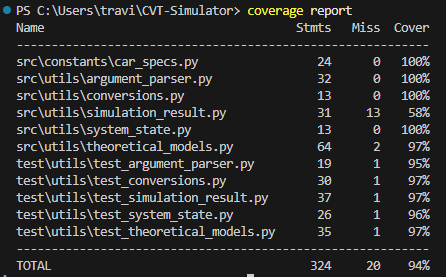
\includegraphics[width=0.7\textwidth]{UnitTestCoverageReport.png}
  \caption{Home Page }
  \label{Fig_Home} 
  \end{center}
\end{figure}


\bibliographystyle{plainnat}
\bibliography{../../refs/References}

\newpage{}
\section*{Appendix --- Reflection}

The information in this section will be used to evaluate the team members on the
graduate attribute of Reflection.

\input{../Reflection.tex}

\begin{enumerate}
  \item What went well while writing this deliverable? 
  \item What pain points did you experience during this deliverable, and how
    did you resolve them?
  \item Which parts of this document stemmed from speaking to your client(s) or
  a proxy (e.g. your peers)? Which ones were not, and why?
  \item In what ways was the Verification and Validation (VnV) Plan different
  from the activities that were actually conducted for VnV?  If there were
  differences, what changes required the modification in the plan?  Why did
  these changes occur?  Would you be able to anticipate these changes in future
  projects?  If there weren't any differences, how was your team able to clearly
  predict a feasible amount of effort and the right tasks needed to build the
  evidence that demonstrates the required quality?  (It is expected that most
  teams will have had to deviate from their original VnV Plan.)
\end{enumerate}

\end{document}